\section{Use Case Model}

\subsection{Use Case Diagrams}

Figures 1 and 2 show two views of the same Room4U boundary. Student and Administrator both use UC-01--UC-03. The Administrator view continues with UC-07--UC-13. Actors represent external roles or systems, not the development team or database.

\begin{figure}[H]
\centering
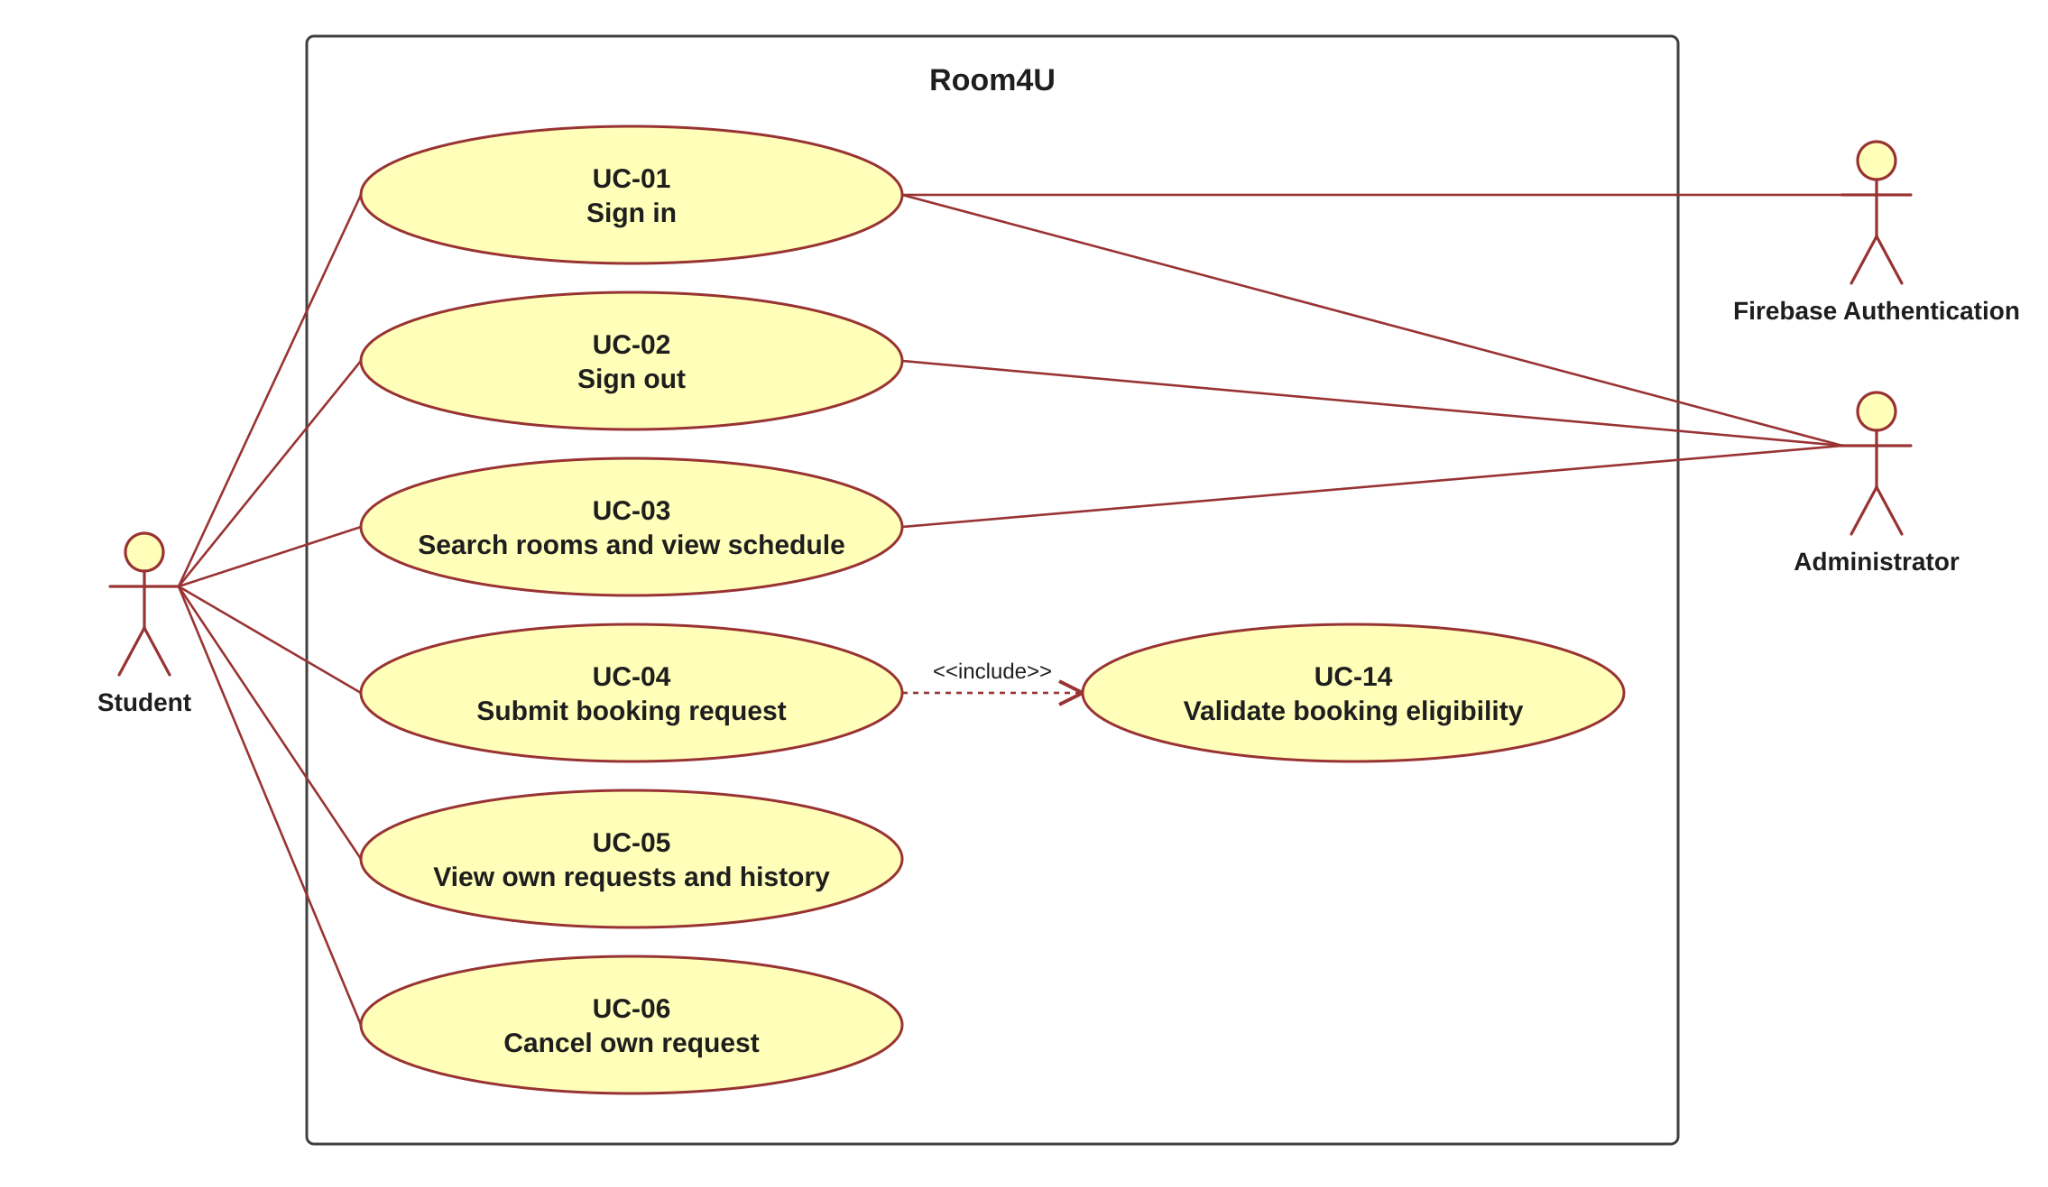
\includegraphics[width=\textwidth,height=0.68\textheight,keepaspectratio]{images/use-case-student.png}
\caption{Student workflows and shared session and room access. The dashed include arrow points from UC-04 to UC-14 because each submission validates eligibility. UC-14 is internal included behavior and has no direct user association. Preconditions such as sign-in are not modeled as repeated include relationships.}
\end{figure}

\begin{figure}[H]
\centering
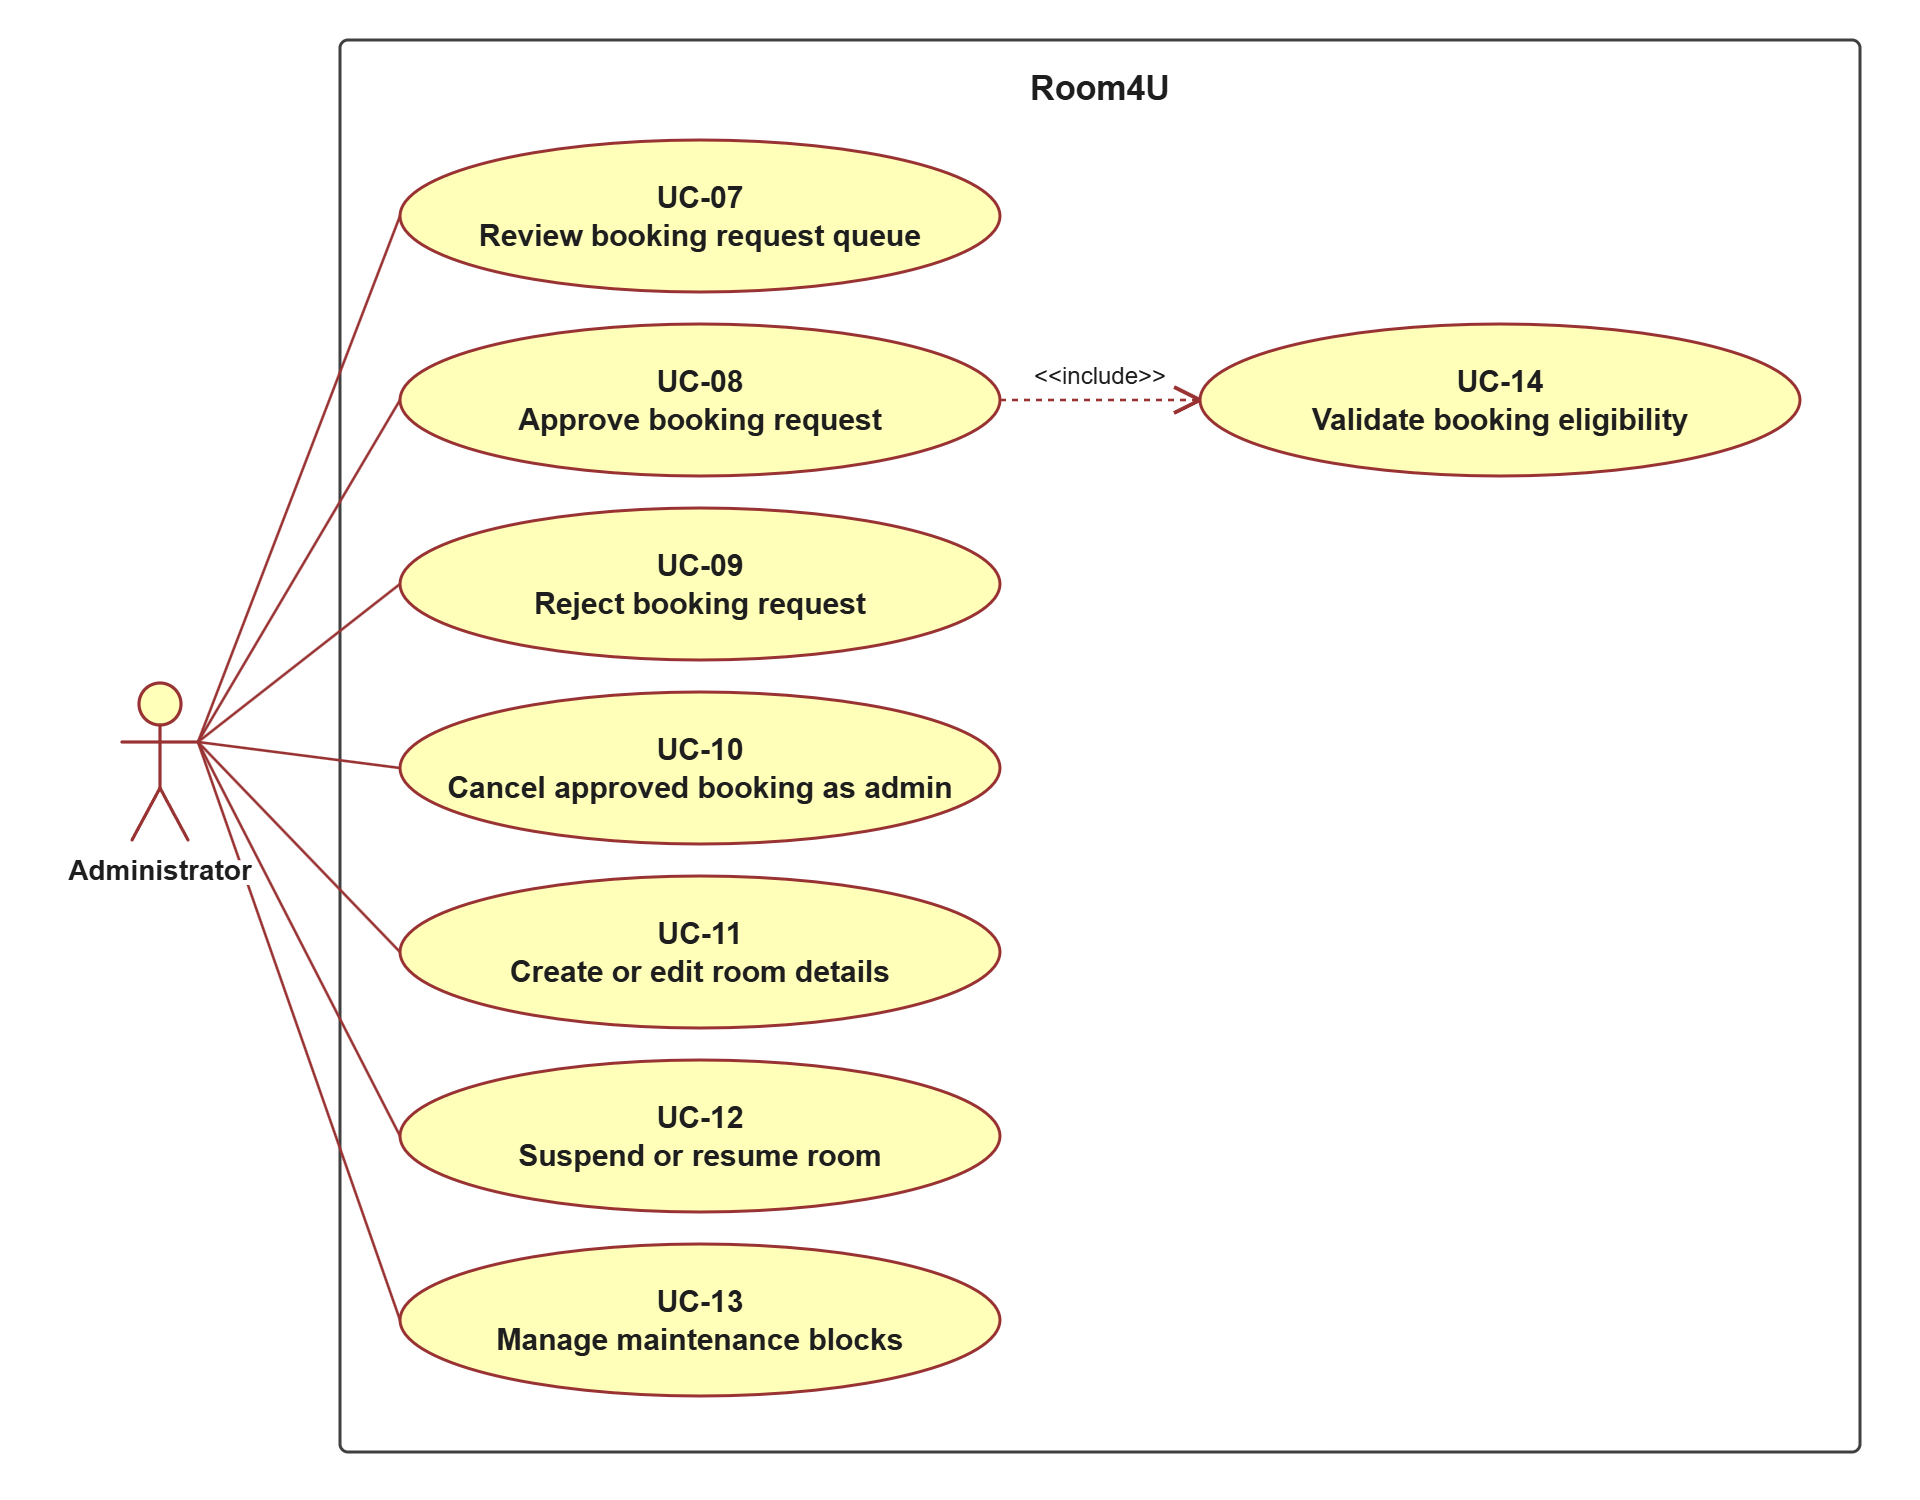
\includegraphics[width=\textwidth,height=0.68\textheight,keepaspectratio]{images/use-case-administrator.png}
\caption{Administrator workflows for requests, rooms and maintenance. UC-08 includes UC-14 for each approval. Rejection, cancellation and maintenance management are separate user goals, not unconditional includes of approval. No extend relationship or actor generalization is needed for the specified behavior.}
\end{figure}

\subsection{Actors}
\begin{srstable}{p{0.25\textwidth}|L}
\textbf{Actor} & \textbf{Responsibilities} \\ \hline
Student & Uses an account created in advance; searches rooms and views schedules; submits, views and cancels only the Student's own booking requests. \\ \hline
Administrator & Reviews, approves, rejects and cancels booking requests; manages rooms and maintenance blocks; and searches rooms and views schedules. An Administrator may work in several windows at the same time. \\ \hline
Firebase Authentication & External system that checks a user's sign-in credentials. It participates in UC-01 only; Room4U determines the user's role and permitted access. \\ \hline
\end{srstable}

The backend and PostgreSQL are internal parts of Room4U, not use-case actors. The instructor and TA are project stakeholders, not product actors.

\subsection{Use Case List}
\begingroup
\small
\setstretch{1.0}
\setlength{\tabcolsep}{3pt}
\renewcommand{\arraystretch}{1.1}
\begin{longtable}{|>{\raggedright\arraybackslash}p{0.40\textwidth}|>{\raggedright\arraybackslash}p{0.20\textwidth}|>{\raggedright\arraybackslash}p{0.12\textwidth}|>{\raggedright\arraybackslash}p{0.23\textwidth}|}
\hline
\textbf{ID and use case} & \textbf{Primary actor} & \textbf{Priority} & \textbf{Related FR} \\ \hline
\endfirsthead
\hline
\textbf{ID and use case} & \textbf{Primary actor} & \textbf{Priority} & \textbf{Related FR} \\ \hline
\endhead
\hline
\endfoot
\hline
\endlastfoot
UC-01 Sign in & Student or Administrator & Must & FR-01--FR-03 \\ \hline
UC-02 Sign out & Student or Administrator & Must & FR-05 \\ \hline
UC-03 Search rooms and view schedule & Student or Administrator & Must & FR-06--FR-09, FR-27 \\ \hline
UC-04 Submit booking request & Student & Must & FR-10--FR-11, FR-19 \\ \hline
UC-05 View own requests and history & Student & Must & FR-04, FR-12, FR-19 \\ \hline
UC-06 Cancel own request & Student & Must & FR-04, FR-13, FR-19 \\ \hline
UC-07 Review booking request queue & Administrator & Must & FR-03, FR-14, FR-19 \\ \hline
UC-08 Approve booking request & Administrator & Must & FR-15--FR-16, FR-19 \\ \hline
UC-09 Reject booking request & Administrator & Must & FR-17, FR-19 \\ \hline
UC-10 Cancel approved booking as administrator & Administrator & Must & FR-18--FR-19 \\ \hline
UC-11 Create or edit room details & Administrator & Must & FR-20--FR-21, FR-27 \\ \hline
UC-12 Suspend or resume room & Administrator & Must & FR-16, FR-22--FR-23, FR-27 \\ \hline
UC-13 Manage maintenance blocks & Administrator & Must & FR-16, FR-24--FR-27 \\ \hline
UC-14 Validate booking eligibility & None (included by UC-04 and UC-08) & Included Must & FR-10, FR-15--FR-16, FR-22 \\ \hline
\end{longtable}
\endgroup

\clearpage